\chapter{Introducción específica}

\label{Chapter2}

En este capítulo se presentan los conceptos técnicos que fundamentan el trabajo: el ciclo de refrigeración y la función del controlador, la arquitectura de conectividad del N150 y las características de BLE (del inglés, \textit{Bluetooth Low Energy}) \cite{bluetooth:core53} relevantes para implementar una interfaz local de comunicación.

%----------------------------------------------------------------------------------------

\section{Ciclo de refrigeración por compresión de vapor}
\label{sec:ciclo_refrigeracion}

Para comprender el entorno de aplicación del controlador N150 y las tareas de soporte asociadas con su operación, resulta necesario introducir el principio de funcionamiento de los sistemas de refrigeración por compresión de vapor, tecnología ampliamente utilizada en heladeras comerciales.

El objetivo de estos sistemas es extraer calor del interior del gabinete refrigerado y disiparlo hacia el ambiente exterior, a fin de mantener una temperatura adecuada para la conservación de los productos almacenados. Para ello, el ciclo se basa en la circulación de un fluido refrigerante a través de un conjunto de componentes, cada uno con una función específica dentro del proceso térmico.

El primer componente del ciclo es el compresor, encargado de aspirar el refrigerante en estado gaseoso y a baja presión desde la salida del evaporador, y comprimirlo hasta alcanzar valores elevados de presión y temperatura. A continuación, el fluido ingresa al condensador, donde cede calor al ambiente y se transforma en líquido a alta presión. Luego atraviesa un dispositivo de expansión, que reduce su presión y temperatura. Finalmente, el refrigerante ingresa al evaporador, donde absorbe calor del interior de la heladera y vuelve a evaporarse, con lo cual se completa el ciclo. Este proceso se representa en la figura \ref{fig:ciclo_refrigeracion}.

\begin{figure}[htbp]
	\centering
	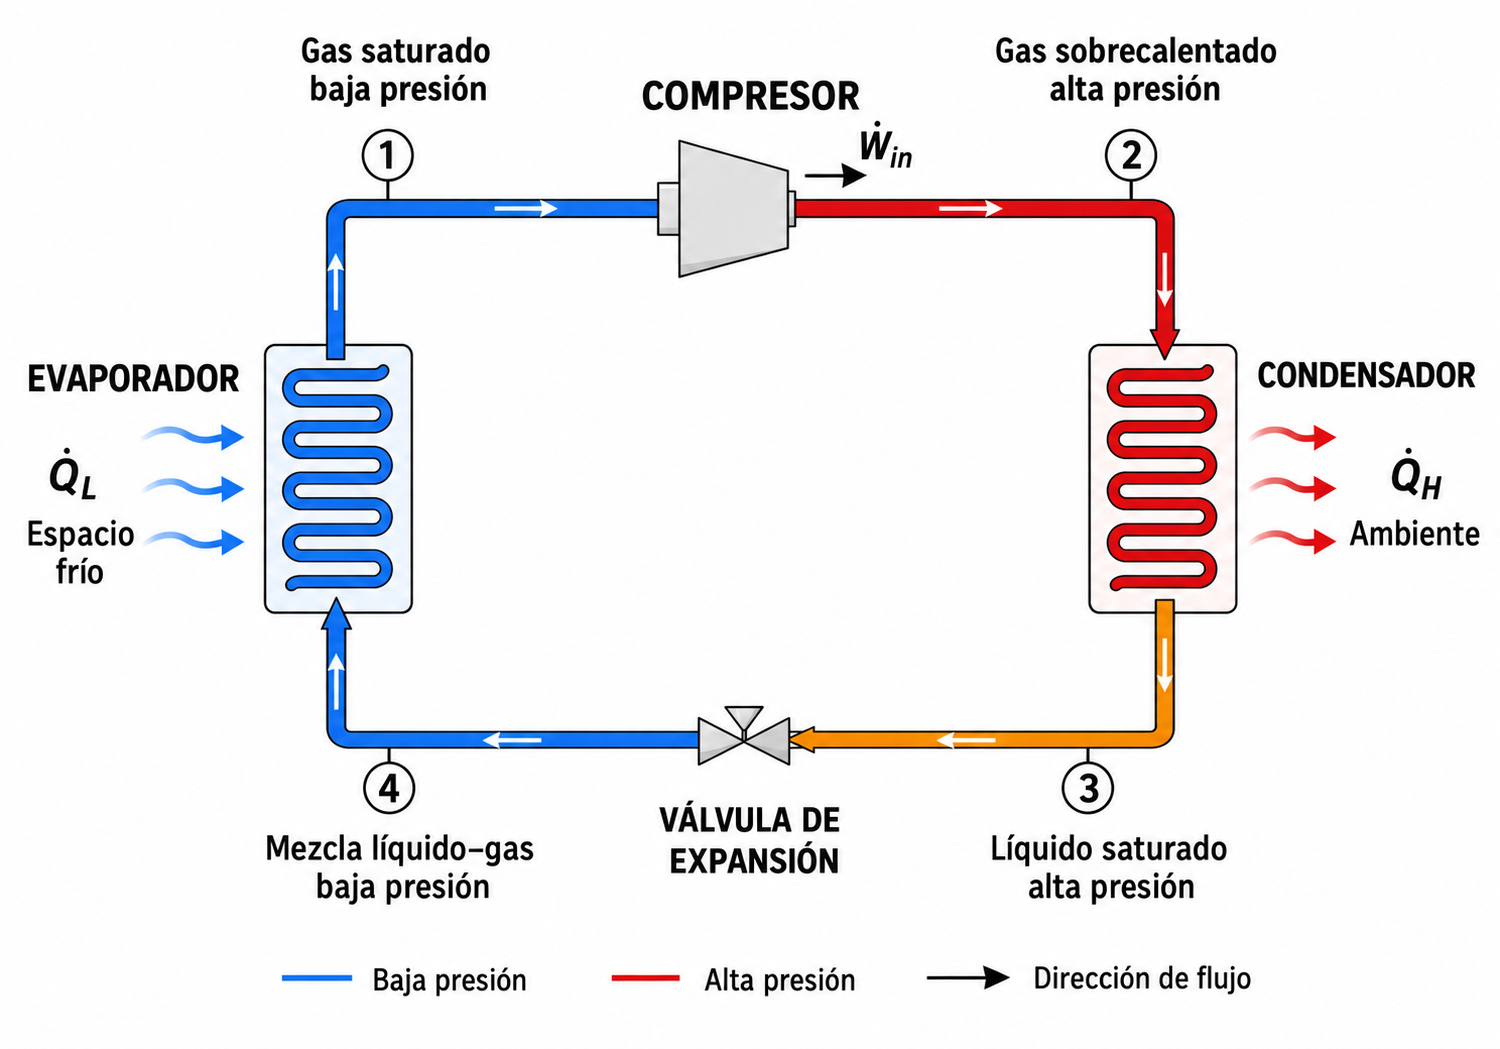
\includegraphics[width=\textwidth]{Figures/cicloRefrigeracion.png}
	\caption[Ciclo de refrigeración]{Esquema del ciclo de refrigeración: compresor, condensador, dispositivo de expansión y evaporador.}
	\label{fig:ciclo_refrigeracion}
\end{figure}

Desde el punto de vista funcional, el desempeño del sistema depende no solo del estado operativo de sus componentes, sino también de la supervisión adecuada de variables como la temperatura, los tiempos de funcionamiento, el estado de los sensores, las maniobras de descongelamiento y la activación de los actuadores. En aplicaciones comerciales, esta supervisión resulta fundamental para garantizar la conservación de los productos, optimizar el consumo energético y detectar fallas de manera temprana.

En el caso particular del N150, el controlador interviene en la lógica de regulación del ciclo de refrigeración y centraliza funciones de supervisión, almacenamiento de eventos, parametrización operativa y conectividad. De este modo, el dispositivo actúa como nexo entre el comportamiento físico del sistema de refrigeración y las funciones de monitoreo, diagnóstico y soporte construidas sobre él.

%----------------------------------------------------------------------------------------

\section{Arquitectura de conectividad del N150}
\label{sec:arquitectura_conectividad}

La arquitectura del N150 distribuye sus funciones entre componentes especializados. El PIC24FJ64GU205T ejecuta la lógica de control del sistema de refrigeración, mientras que el ESP32 administra las comunicaciones y vincula el sistema de control con las interfaces local y remota. Esta separación evita que las tareas de conectividad interfieran con las funciones de regulación y permite modificar los mecanismos de comunicación sin alterar la lógica principal del equipo.

La comunicación remota se realiza mediante un módem celular Quectel BG95, controlado por el ESP32 a través de una interfaz serie y comandos AT. Esta interacción permite inicializar el módulo, verificar el estado de la tarjeta SIM, registrar el equipo en la red, establecer la conexión de datos y transmitir información hacia la infraestructura de Sensify. La disponibilidad del enlace depende de la cobertura de las redes celulares admitidas por la variante del módem instalada.

Para el acceso local se utiliza la interfaz BLE integrada en el ESP32 y gestionada mediante ESP-IDF 5.3.3. Este canal permite que un teléfono se comunique directamente con el controlador sin utilizar el módem celular ni una red del establecimiento. La figura \ref{fig:conexion_N150} presenta la relación entre los componentes y los canales de comunicación del N150.

\begin{figure}[htbp]
	\centering
	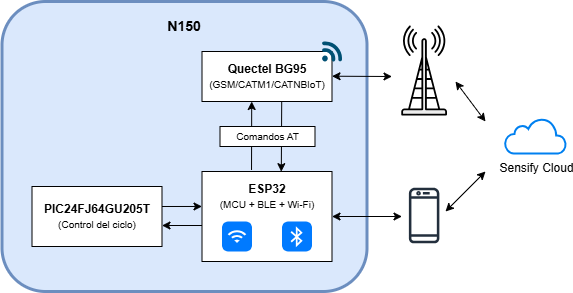
\includegraphics[width=\textwidth]{Figures/conexionN150.png}
	\caption[Arquitectura de conectividad del N150]{Arquitectura de conectividad del controlador N150.}
	\label{fig:conexion_N150}
\end{figure}

%----------------------------------------------------------------------------------------

\section{Bluetooth Low Energy}
\label{sec:ble}

BLE es una tecnología inalámbrica de corto alcance orientada al intercambio eficiente de cantidades moderadas de datos. Su especificación define, entre otros elementos, los procedimientos de descubrimiento y conexión, los roles de los dispositivos y el modelo utilizado para organizar la información intercambiada. La documentación de ESP-IDF 5.3.3 describe el soporte provisto por el ESP32 para implementar estos mecanismos \cite{espressif:esp-idf-ble}. Para este trabajo no resultan relevantes todas las capas del protocolo, sino aquellas que permiten establecer una comunicación directa y segura entre el N150 y un teléfono.

\subsection{Adecuación de BLE al N150}
\label{subsec:seleccion_ble}

Para el desarrollo se requería un canal local que permitiera configurar el controlador, consultar información de diagnóstico y actualizar su firmware aun cuando la heladera estuviera instalada en un sitio sin cobertura celular. También debía posibilitar el uso de un teléfono como herramienta de soporte, sin incorporar hardware adicional al N150. BLE satisface estos requerimientos porque se encuentra integrado en el ESP32, dispone de soporte en dispositivos móviles y permite descubrir y conectar equipos cercanos sin depender de una infraestructura de red externa.

El alcance acotado de BLE también resulta coherente con las tareas de intervención local, en las que el operador se encuentra próximo a la heladera. El caudal disponible es suficiente para intercambiar parámetros, estados, registros de diagnóstico y bloques de una actualización de firmware. Además, su modelo de servicios y características permite organizar esas operaciones mediante una interfaz común para el controlador y la aplicación móvil.

La tabla \ref{tab:requerimientos_ble} relaciona las necesidades principales de la interfaz local con las características de BLE aprovechadas en el desarrollo. Esta correspondencia permite justificar la selección a partir de los requerimientos del sistema y no solo de las propiedades generales de la tecnología.

\begin{table}[htbp]
	\centering
	\caption{Relación entre los requerimientos de la interfaz local y las características de BLE.}
	\begin{tabular}{p{0.34\textwidth} p{0.56\textwidth}}
		\toprule
		\textbf{Requerimiento} & \textbf{Característica utilizada} \\
		\midrule
		Operación sin cobertura celular & Enlace directo entre el teléfono y el N150, independiente de servicios externos. \\
		Uso de un teléfono como herramienta & Compatibilidad de BLE con dispositivos móviles y mecanismos de descubrimiento de equipos próximos. \\
		Ausencia de hardware adicional & Interfaz de radio integrada en el ESP32 del controlador. \\
		Configuración y diagnóstico & Organización de datos y operaciones mediante servicios y características GATT. \\
		Actualización de firmware & Transferencia bidireccional de bloques de datos durante una conexión establecida. \\
		Control de acceso & Emparejamiento, autenticación y cifrado del enlace. \\
		\bottomrule
	\end{tabular}
	\label{tab:requerimientos_ble}
\end{table}

Frente a la conectividad celular, BLE proporciona acceso cuando no existe cobertura o cuando el enlace remoto no se encuentra disponible. A diferencia de Wi-Fi, no requiere que el controlador se incorpore a una red local ni que se conozcan sus credenciales. Por otra parte, ofrece una sesión de comunicación y un modelo de datos más apropiados para las tareas previstas que una interfaz de proximidad basada en NFC. Bluetooth Classic proporciona un caudal mayor, pero ese beneficio no resulta necesario para el volumen de información de esta aplicación. Por estos motivos, se seleccionó BLE como interfaz local del N150.

\subsection{Comunicación entre el teléfono y el controlador}
\label{subsec:comunicacion_ble}

La comunicación comienza con la emisión periódica de paquetes de publicidad por parte del N150. El teléfono explora los dispositivos cercanos, identifica el controlador y solicita el establecimiento de una conexión, de acuerdo con el flujo previsto por la plataforma para el descubrimiento y la conexión BLE \cite{espressif:esp-idf-ble}. En este esquema, el N150 funciona como periférico y el teléfono como central. La publicidad permite iniciar la comunicación sin conocer previamente la dirección del dispositivo y limita la búsqueda al entorno próximo del operador.

La sesión de soporte local se divide en tres etapas. En la primera, la aplicación identifica el N150 mediante la información incluida en sus paquetes de publicidad. En la segunda, ambos dispositivos establecen la conexión y aplican los mecanismos de seguridad previstos para verificar el acceso. En la tercera, la aplicación descubre la interfaz GATT y ejecuta la operación solicitada. Esta secuencia se utiliza tanto para intervenciones breves, como la consulta de un estado, como para operaciones prolongadas, entre ellas la transferencia de una actualización de firmware.

Una vez establecida la conexión, los datos se intercambian mediante GATT (del inglés, \textit{Generic Attribute Profile}). El N150 funciona como servidor GATT y expone la información y las operaciones disponibles mediante servicios y características. El teléfono funciona como cliente GATT, descubre esa estructura y accede a ella de acuerdo con los permisos definidos.

Los roles de conexión y los roles GATT describen aspectos diferentes y complementarios. La condición de periférico establece la participación del N150 en el descubrimiento y en la conexión BLE, mientras que la condición de servidor determina que conserva y expone los atributos. De manera análoga, el teléfono actúa como central porque inicia la conexión y como cliente porque solicita operaciones sobre los atributos publicados por el controlador.

La interfaz implementada utiliza las cuatro operaciones de acceso requeridas por el sistema: lectura, escritura, notificación e indicación. Las lecturas permiten que el teléfono solicite valores al controlador y las escrituras permiten enviarle datos o comandos. Las notificaciones y las indicaciones posibilitan que el N150 informe cambios o resultados sin esperar una consulta periódica; las indicaciones, a diferencia de las notificaciones, requieren confirmación de recepción. Estas operaciones sustentan las funciones de parametrización, diagnóstico y actualización de firmware desarrolladas para la aplicación móvil.

Debido a que la interfaz permite modificar la configuración y el firmware del controlador, el acceso no puede depender únicamente de la proximidad física. Por este motivo, la comunicación incorpora mecanismos de emparejamiento, autenticación y cifrado del enlace. De esta manera, BLE proporciona tanto el canal local requerido para las tareas de soporte como los mecanismos necesarios para restringir el acceso a las funciones del N150.
